\setcounter{ex}{0}
\section{Khảo sát và vẽ đồ thị hàm số}
\subsection{Đề 1}
\Opensolutionfile{ans}[ans/ans-2-B4-De1-NLC]
\caulc
\begin{ex}%[2D1N4-3]
	\immini[thm]
	{	Cho hàm số $y=f(x)$ có đồ thị như hình bên.
		Phương trình các đường tiệm cận của đồ thị hàm số $y=f(x)$ là
		\choice[2]
		{$x=1$ và $y=-2$}
		{$x=1$ và $y=2$}
		{$x=-1$ và $y=-2$}
		{\True $x=-1$ và $y=2$}}
		{	\begin{tikzpicture}[line join = round, line cap = round,>=stealth,x = 1cm,y = 1cm,font=\footnotesize,scale=.6] 
				%Nhập các thông số ban đầu 
				\def\xmin{-4.5}		\def\xmax{3} 
				\def\ymin{-3}		\def\ymax{6} 
				\def\hamso{(2*\x +3)/((\x)+1)} 
				\pgfmathsetmacro{\tiemcanngang}{2} 
				%Vẽ hệ trục Oxy 
				\draw[->] (\xmin,0)--(0,0) node[below right]{$O$}--(\xmax,0) node[below]{$x$}; 
				\draw[->] (0,\ymin)--(0,\ymax) node[right]{$y$}; 
				\fill (0,0) circle (1.5pt); 
				%Vẽ các điểm trên hệ trục 
				\draw (-1,0) circle (1pt) node[below right] {$-1$}  (0,2) circle (1pt) node[below right] {$2$}  (0,3) circle (1pt) node[above right] {$3$};
				%Vẽ đồ thị hàm số 
				\begin{scope} 
					\clip (\xmin,\ymin) rectangle (\xmax,\ymax); 
					\draw[samples=300,domain=\xmin:\xmax,smooth] plot (\x, {\hamso}); 
				\end{scope} 
				%Vẽ tiệm cận ngang 
				\draw[smooth,blue!50!black](\xmin,\tiemcanngang)--(\xmax,\tiemcanngang); 
			\end{tikzpicture}}
	\loigiai{
		Dựa vào đồ thị, ta suy ra tiệm cận đứng và tiệm cận ngang của đồ thị lần lượt là các đường thẳng $x=-1$, $y=2$.
	}
\end{ex}

\begin{ex}%[2D1N4-3]
	\immini[thm]
	{	Cho hàm số $y=f(x)$ có đồ thị như hình bên.
		Tổng số tiệm cận đứng và tiệm cận ngang của đồ thị hàm số $y=f(x)$ là
		\choice[2]
		{$4$}
		{\True $3$}
		{$2$}
		{$1$}}
		 	{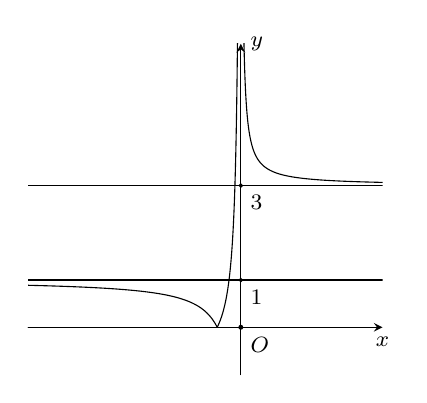
\begin{tikzpicture}[line join = round, line cap = round,>=stealth,x = 1cm,y = 1cm,font=\footnotesize,scale=.6] 
		 			%Nhập các thông số ban đầu 
		 			\def\xmin{-4.5}		\def\xmax{3} 
		 			\def\ymin{-1}		\def\ymax{6} 
		 			\draw[->] (\xmin,0)--(0,0) node[below right]{$O$}--(\xmax,0) node[below]{$x$}; 
		 			\draw[->] (0,\ymin)--(0,\ymax) node[right]{$y$}; 
		 			\fill (0,0) circle (1.5pt); 
		 			\draw (0,1) circle (1pt) node[below right] {$1$} (0,3) circle (1pt) node[below right] {$3$};
		 			%Vẽ đồ thị hàm số 
		 			\clip (\xmin,\ymin) rectangle (\xmax,\ymax);
		 			\draw[samples=300,domain=0.001:\xmax,smooth] plot (\x, {(15*\x+1)/(5*\x)}); 
		 			\draw[samples=300,domain=\xmin:-.5,smooth] plot (\x, {(2*\x+1)/(2*\x)}); 
		 			\draw[samples=300,domain=-.5:0,smooth] plot (\x, {(-2*\x-1)/(2*\x)}); 
		 			%Vẽ tiệm cận ngang 
		 			\draw[smooth](\xmin,1)--(\xmax,1); 
		 			\draw[smooth](\xmin,3)--(\xmax,3); 
		 	\end{tikzpicture}}
	 \loigiai{
		Dựa vào đồ thị của hàm số $y=f(x)$ ta có
		\begin{itemize}
			\item $\lim\limits_{x \to-\infty} f(x)=1$ nên đường thẳng $y=1$ là một đường tiệm cận ngang của đồ thị hàm số $y=f(x)$.
			\item $\lim\limits_{x \to +\infty} f(x)=3$ nên đường thẳng $y=3$ là một đường tiệm cận ngang của đồ thị hàm số $y=f(x)$.
			\item $\lim\limits _{x \to 0^{-}} f(x)=+\infty$ và $\lim\limits_{x \to 0^{+}} f(x)=+\infty$ suy ra đường thẳng $x=0$ là tiệm cận đứng của đồ thị hàm số $y=f(x)$.
		\end{itemize}
		Vậy đồ thị hàm số $y=f(x)$ có tất cả $3$ đường tiệm cận.
		}
\end{ex}

\begin{ex}%[2D1N4-3]
	\immini[thm]
	{Cho hàm số $y=f(x)$ có đồ thị như hình bên.
		Đồ thị hàm số đã cho có bao nhiêu đường tiệm cận? 
		\choice[2]
		{$4$}
		{\True $2$}
		{$1$}
		{$3$}}
		 {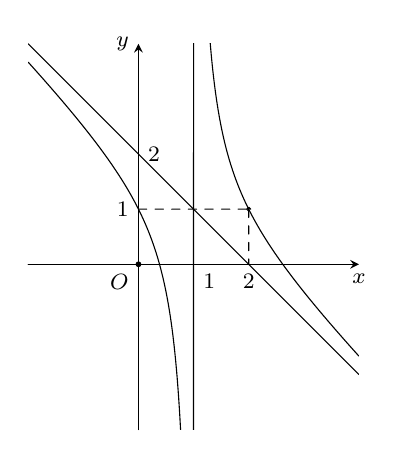
\begin{tikzpicture}[line join = round, line cap = round,>=stealth,x = 1cm,y = 1cm,font=\footnotesize,scale=.7] 
		 		%Nhập các thông số ban đầu 
		 		\def\xmin{-2}		\def\xmax{4}  
		 		\def\ymin{-3}		\def\ymax{4}  
		 		\def\hamso{(-(\x)^2+3*\x-1)/((\x)-1)}  
		 		\def\tiemcanxien{(-1)*\x +2}  
		 		%Vẽ hệ trục Oxy 
		 		\draw[->] (\xmin,0)--(0,0) node[below left]{$O$}--(\xmax,0) node[below]{$x$}; 
		 		\draw[->] (0,\ymin)--(0,\ymax) node[left]{$y$}; 
		 		\fill (0,0) circle (1.5pt); 
		 		%Vẽ các điểm gióng 
		 		\draw (1,0) node[below right] {$1$}(0,2) node [right] {$2$};
		 		\draw[dashed] (0,1) node[left]{$1$}--(2,1) circle (1pt)--(2,0) node [below] {$2$};
		 		%Vẽ đồ thị hàm số và tiệm cận xiên 
		 		\begin{scope} 
		 			\clip (\xmin,\ymin) rectangle (\xmax,\ymax); 
		 			\draw[samples=250,domain=\xmin:\xmax,smooth] plot (\x, {\hamso}); %Đồ thị hàm số 
		 			\draw[samples=250,domain=\xmin:\xmax,smooth] plot (\x, {\tiemcanxien}); %Tiệm cận xiên 
		 		\end{scope} 
		 \end{tikzpicture}}
 	 \loigiai{
 	 	Từ đồ thị hàm số ta thấy hàm số đã cho có $1$ tiệm cận đứng và $1$ tiệm cận xiên.
	}
\end{ex}

\begin{ex}%[2D1N4-1]
	Cho hàm số $y=f(x)$ có bảng biến thiên như sau
	\begin{center}
		
\begin{tikzpicture}
			\tkzTabInit[nocadre,lgt=1.2,espcl=4]
			{$x$/1,$f’(x)$/1,$f(x)$/2}
			{$-\infty$,$1$,$+\infty$}
			\tkzTabLine{ ,+,z,-, }
			\tkzTabVar{-/$1$,+D+/$10$/$3$ ,-/$-\infty$}
		\end{tikzpicture}.
	\end{center}
	Tổng số tiệm cận ngang và tiệm cận đứng của đồ thị hàm số đã cho là
	\choice 
		{$4$}
		{\True $1$}
		{$3$}
		{$2$}
	\loigiai{
		Dựa vào bảng biến thiên của hàm số ta thấy
		\begin{itemize}
			\item $\lim\limits_{x \to +\infty} y=-\infty$ và $\lim\limits_{x \to -\infty} y=1$ nên đường thẳng $y=1$ là tiệm cận ngang của đồ thị hàm số.
			\item $\lim\limits_{x \to 1^{+}} y=3$ và $\lim\limits_{x \to 1^{-}} y=10$ nên đường thẳng $x=1$ không là tiệm cận đứng của đồ thị hàm số.
		\end{itemize}		
	Vậy hàm số đã cho có tổng số tiệm cận đứng và tiệm cận ngang là $1$.
	}
\end{ex}

\begin{ex}%[2D1N4-1]
	 Đồ thị hàm số nào sau đây nhận đường thẳng $x=2$ là tiệm cận đứng?
	 \choice 
		 {\True $y=\dfrac{2 x}{x-2}$}
		 {$y=2$}
		 {$y=\dfrac{2 x}{x+2}$}
		 {$y=x-2-\dfrac{2}{x}$}
 	\loigiai{
	 	Xét hàm số $y=\dfrac{2x}{x-2}$ ta có
	 	\begin{itemize}
	 		\item Tập xác định $\mathscr{D}=\mathbb{R} \setminus\{2\}$.
	 		\item $\lim\limits_{x \to 2^{+}} \dfrac{2 x}{x-2}=+\infty$ và $\lim\limits_{x \to 2^{-}} \dfrac{2 x}{x-2}=-\infty$.
	 	\end{itemize}  
	    Vậy đồ thị hàm số $y=\dfrac{2 x}{x-2}$ có tiệm cận đứng là $x=2$.
	}
\end{ex}

\begin{ex}%[2D1N4-1]
	Cho hàm số $y=f(x)$ có đạo hàm trên $\mathbb{R}\setminus\{ \pm 1\}$ và có bảng biến thiên như hình vẽ dưới đây 
	\begin{center}
		
\begin{tikzpicture}
		\tkzTabInit[nocadre,lgt=1.5,espcl=2,deltacl=.5]
		{$x$/0.7, $f(x)$/0.7, $f(x)$/2}
		{$-\infty$,$-1$,$0$,$1$,$+\infty$}
		\tkzTabLine{,+,d,-,z,+,d,+,}
		\tkzTabVar{-/$-3$ ,+D+/$1$/$+\infty$ ,-/ $-2$, +D-/$+\infty$/$-\infty$,+/$3$}
		\end{tikzpicture}.
	\end{center}
	Hỏi hàm số $y=f(x)$ có tất cả bao nhiêu đường tiệm cận?
	\choice 
		{$1$}
	 	{\True $4$}
	 	{$3$}
	 	{$2$}
 	\loigiai{
 		Dựa vào bảng biến thiên của hàm số ta thấy
 		\begin{itemize}
 			\item $\lim\limits_{x\to +\infty}f(x)=3$, $\lim\limits_{x\to -\infty}f(x)=-3$, suy ra đồ thị hàm số có $2$ tiệm cận ngang là $y=3$ và $y=-3$.
 			\item $\lim\limits_{x\to -1^+}f(x)=+\infty$, $\lim\limits_{x\to 1^-}f(x)=+\infty$, $\lim\limits_{x\to 1^+}f(x)=-\infty$, suy ra đồ thị hàm số có $2$ tiệm cận đứng là $x=-1$ và $x=1$.
 		\end{itemize} 
 		 Vậy hàm số có tất cả $4$ đường tiệm cận.
	}
\end{ex}

\begin{ex}%[2D1N4-1]
	Cho hàm số $f(x)$ có bảng biến thiên như sau
	\begin{center}
		
\begin{tikzpicture}
			\tkzTabInit[nocadre,lgt=1.2,espcl=2,deltacl=.5]
			{$x$/0.7, $f(x)$/0.7, $f(x)$/2}
			{$-\infty$,$0$,$3$,$+\infty$}
			\tkzTabLine{,-,d,-,z,+,}
			\tkzTabVar{+/$1$ ,-D+/$-\infty$/$2$ ,-/ $-3$, +/$3$}
		\end{tikzpicture}.
	\end{center}
	Tổng số tiệm cận đứng và tiệm cận ngang của đồ thị hàm số đã cho là 
	\choice 
		{$1$}
		{$2$}
		{\True $3$}
		{$4$}
	\loigiai{
	Dựa vào bảng biến thiên của hàm số ta có
	\begin{itemize}
		\item $\lim\limits_{x \to +\infty} y=3$ và $\lim\limits_{x \to -\infty} y=1$ nên đồ thị hàm số có hai tiệm cận ngang $y=1$, $y=3$.
		\item $\lim\limits_{x \to 0^{-}} y=-\infty$ nên đồ thị hàm số có tiệm cận đứng $x=0$.
	\end{itemize} 
	 Vậy đồ thị hàm số có tổng cộng $3$ đường tiệm cận.
	}
\end{ex}

\begin{ex}%[2D1N4-1]
	Cho hàm số $y=f(x)$ có bảng biến thiên như sau
	\begin{center}
		\begin{tikzpicture}
		\tkzTabInit[nocadre,lgt=1.2,espcl=3,deltacl=0.5]
		{$x$/.7, $f(x)$/.7, $f(x)$/2}
		{$-\infty$,$-3$,$3$,$+\infty$}
		\tkzTabLine{,+,d,+,d,+,}
		\draw ($(N12)!0.5!(N13)$) node(A){$0$} (N22) node[below left] (B){$+\infty$} (N23)
		node[above right](C){$-\infty$} (N32)
		node[below left](D){$+\infty$} (N33)
		node[above right](E){$-\infty$} ($(N42)!0.5!(N43)$)
		node(F){$0$};
		\draw[-stealth] (A)--(B);
		\draw[-stealth] (C)--(D);
		\draw[-stealth] (E)--(F);
		\draw[double] ([yshift=-1mm]N22)--(N23);
		\draw[double] ([yshift=-1mm]N32)--(N33);
		\end{tikzpicture}.
	\end{center}
	Số đường tiệm cận của đồ thị hàm số đã cho là
	\choice 
		{\True $3$}
		{$1$}
		{$4$}
		{$2$}
	\loigiai{
	Dựa vào bảng biến thiên của hàm số ta có
	\begin{itemize}
		\item $\lim\limits_{x \to \pm \infty} y=0 \Rightarrow y=0$ là đường tiệm cận ngang.
		\item $\lim\limits_{x \to (-3)^{+}} y=-\infty \Rightarrow x=-3$ là đường tiệm cận đứng.
		\item $\lim\limits_{x \to 3^{+}} y=-\infty \Rightarrow x=3$ là đường tiệm cận đứng.
	\end{itemize}
 	 Vậy số đường tiệm cận của đồ thị hàm số đã cho là $3$.
	}
\end{ex}

\begin{ex}%[2D1H5-7]
	Đồ thị hàm số nào dưới đây có tâm đối xứng là điểm $I(1;-2)$?
	\choice 
		{$y=\dfrac{2x-3}{2 x+4}$}
		{\True $y=2x^3-6 x^2+x+1$}
		{$y=-2x^3+6 x^2+x-1$}
		{$y=\dfrac{2-2x}{1-x}$}
	\loigiai{
		Hàm số $y=2x^3-6x^2+x+1$ có $y'=6x^2-12 x+1$ và $y''=12 x-12$.\\
		Xét phương trình $y''=0 \Leftrightarrow 12 x-12=0\Leftrightarrow x=1$. Đồ thị hàm số có điểm uốn $I(1;-2)$ là tâm đối xứng của đồ thị hàm số.
	}
\end{ex}

\begin{ex}%[2D1H5-7]
	Tâm đối xứng của đồ thị hàm số $y=x^3-6 x^2+x+1$ là điểm nào trong các điểm sau?
	\choice 
		{$I(2;13)$}
		{\True $I(2;-13)$}
		{$I(-2;-13)$}
		{$I(-2;-33)$}
 	\loigiai{
 		Ta có $y'=3 x^2-12 x+1 \Rightarrow y''=6 x-12$. Do đó $y''=0 \Leftrightarrow x=2 \Rightarrow y=-13$.\\
		Tâm đối xứng của đồ thị hàm số $y=x^3-6 x^2+x+1$ là $I(2;-13)$.
	}
\end{ex}

\begin{ex}%[2D1H4-1]
	\immini[thm]
	{Cho hàm số $y=f(x)$ có đồ thị như hình bên.
		Đồ thị hàm số đã cho có bao nhiêu đường tiệm cận? 
		\choice[2] 
		{\True $4$}
		{$2$}
		{$1$}
		{$3$}}
		{	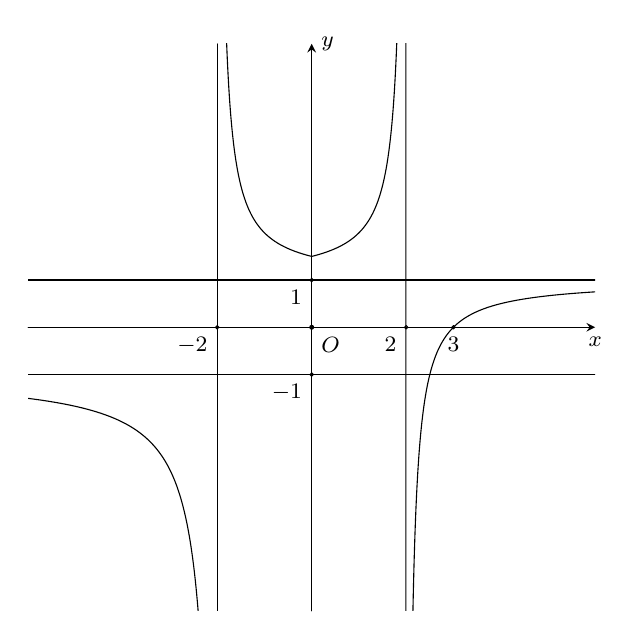
\begin{tikzpicture}[line join = round, line cap = round,>=stealth,x = 1cm,y = 1cm,font=\footnotesize,scale=.6] 
				%Nhập các thông số ban đầu 
				\def\xmin{-6}		\def\xmax{6} 
				\def\ymin{-6}		\def\ymax{6} 
				\def\tcd{-2}
				\draw[->] (\xmin,0)--(0,0) node[below right]{$O$}--(\xmax,0) node[below]{$x$}; 
				\draw[->] (0,\ymin)--(0,\ymax) node[right]{$y$}; 
				\fill (0,0) circle (1.5pt); 
				%Vẽ các điểm trên hệ trục 
				\draw (-2,0) circle (1pt) node[below left]{$-2$} (2,0) circle (1pt) node[below left]{$2$} (3,0) circle (1pt) node[below ]{$3$} (0,1) circle (1pt) node[below left]{$1$} (0,-1) circle (1pt) node[below left]{$-1$};
				%Vẽ đồ thị hàm số 
				\clip (\xmin,\ymin) rectangle (\xmax,\ymax);
				\draw[samples=300,domain=0:\xmax,smooth] plot (\x, {(\x-3)/(\x-2)}); 
				\draw[samples=300,domain=\xmin:-2.1,smooth] plot (\x, {(-50*\x+1)/(50*\x+100)});
				\draw[samples=300,smooth,domain=-1.9:0] plot (\x, {(\x+3)/(\x+2)}); 
				\draw(-2,\ymin)--(-2,\ymax);
				%Vẽ tiệm cận ngang 
				\draw(\xmin,-1)--(\xmax,-1); 
				\draw(\xmin,1)--(\xmax,1); 
		\end{tikzpicture}}
	\loigiai{
		Từ đồ thị hàm số ta thấy
		\begin{itemize}
			\item $\lim\limits_{x \to -\infty} f(x)=-1$ nên đường thẳng $y=-1$ là một đường tiệm cận ngang.
			\item $\lim\limits_{x \to +\infty} f(x)=1$ nên đường thẳng $y=1$ là một đường tiệm cận ngang.
			\item $\lim\limits_{x \to -2^{+}} f(x)=+\infty$ và $\lim\limits_{x \to -2^{-}} f(x)=-\infty$ nên đường thẳng $x=-2$ là đường tiệm cận đứng.
			\item $\lim\limits_{x \to 2^{-}} f(x)=+\infty$ và và $\lim\limits_{x \to 2^{+}} f(x)=-\infty$ nên đường thẳng $x=-2$ là đường tiệm cận đứng.
		\end{itemize}
	Vậy đồ thị hàm số có $4$ đường tiệm cận.
	}
\end{ex}

\begin{ex}%[2D1H4-1]
	Cho hàm số $y=f(x)$ có bảng biến thiên như sau
	\begin{center}
		\begin{tikzpicture}
			\tkzTabInit[nocadre,lgt=1.2,espcl=3,deltacl=0.5]
			{$x$/.7, $f(x)$/.7, $f(x)$/2}
			{$-\infty$,$0$,$3$,$+\infty$}
			\tkzTabLine{,+,z,-,z,+,}
			\draw (N13) node[above] (A) {$-\infty$} (N22) node [below] (B) {$4$} ($(N32)!0.5!(N33)$) node (C) {$-1$} (N42) node[below] (D){+$\infty$};
			\draw[-stealth] (A)--(B);
			\draw[-stealth] (B)--(C);
			\draw[-stealth] (C)--(D);
		\end{tikzpicture}
	\end{center}
	Mệnh đề nào sau đây \textbf{đúng}?
	\choice 
		{Đồ thị hàm số có $2$ đường tiệm cận ngang}
		{Đồ thị hàm số có đường tiệm cận ngang $y=4$}
		{\True Đồ thị hàm số không có tiệm cận} 
		{Đồ thị hàm số có đường tiệm cận đứng $x=0$}
	\loigiai{
		Từ bảng biến thiên của hàm số $y=f(x)$ ta có
		\begin{itemize}
			\item $\lim\limits_{x \to -\infty} f(x)=-\infty, \lim\limits_{x \to +\infty} f(x)=+\infty$ nên đồ thị hàm số đã cho không có tiệm cận ngang.
			\item $\lim\limits_{x \to 0^{+}} f(x)=4, \lim\limits_{x \to 0^{-}} f(x)=4, \lim\limits_{x \to 3^{-}} f(x)=-1, \lim\limits_{x \to 3^{+}} f(x)=-1$ nên đồ thị hàm số đã cho không có tiệm cận đứng.
		\end{itemize}
		Vậy đồ thị hàm số đã cho không có tiệm cận.
	}
\end{ex}
\Closesolutionfile{ans}
\indapan{6}{ans/ans-2-B4-De1-NLC}

\cauds
\Opensolutionfile{ans}[ans/ans-2-B4-De1-DS]
\begin{ex}%[2D1V1-3]
	Cho hàm số $f(x)=\dfrac{x+4}{x-m}$ (với $m$ là tham số thực).
	\choiceTF 
		{Hàm số nghịch biến trên $\mathbb{R}$} {Hàm số có một cực trị}
		{Nếu $m<-4$ thì hàm số nghịch biến trên khoảng $(-\infty;m)$ và $(m;+\infty)$} 
		{\True Có $10$ giá trị nguyên của $m$ để hàm số nghịch biến trên khoảng $(6 ;+\infty)$}
	\loigiai{
			Tập xác định của hàm số là $\mathscr{D}=(-\infty;m) \cup(m;+\infty)$. \\
			Ta có $f'(x)=\left(\dfrac{x+4}{x-m}\right)'=\dfrac{-m-4}{(x-m)^2}$, $\forall x\in \mathscr{D}$.
		\begin{itemchoice}
			\itemch \textbf{Sai}. Hàm số không xác định trên $\mathbb{R}$ nên hàm số không nghịch biến trên $\mathbb{R}$. 
			\itemch \textbf{Sai}. Do $f'(x)$ không đổi dấu trên $\mathscr{D}$ nên hàm số không có cực trị.
			\itemch \textbf{Sai}. Nếu $m<-4$ thì $f'(x)=\dfrac{-m-4}{(x-m)^2}>0$, $\forall x\in \mathscr{D}$ nên hàm số không nghịch biến trên khoảng $(-\infty;m)$ và $(m;+\infty)$.
			\itemch \textbf{Đúng}. Để hàm số $f(x)=\dfrac{x+4}{x-m}$ nghịch biến trên khoảng $\left( 6 ;+\infty\right)$ ta cần $$\heva{&f'(x)<0 \\ &m \notin(6 ;+\infty)} \Rightarrow\heva{&-m-4<0 \\ &m \le 6}\Rightarrow-4<m \le 6.$$ Vì $m$ nguyên nên $m \in\{-3;-2;-1;0;1;2;3;4;5;6\}$.\\
			Vậy có $10$ giá trị nguyên của $m$ để hàm số nghịch biến trên khoảng $(6 ;+\infty)$.
		\end{itemchoice}
}
\end{ex}

\begin{ex}%[2D1V2-2]
	Cho hàm số $f(x)$, bảng xét dấu của $f'(x)$ như sau 
	\begin{center}
		
\begin{tikzpicture}
			\tkzTabInit[lgt=1.2,espcl = 3]
			{$x$ /.7, $f'(x)$ /.7}
			{$-\infty$,$-3$,$-1$,$1$,$+\infty$}
			\tkzTabLine{ ,-,z,+,z,-,z,+, }
		\end{tikzpicture}.
	\end{center}	
	\choiceTF 
		{\True Hàm số có ba điểm cực trị}
		{Hàm số nghịch biến trên khoảng $(-3 ;-1)$}
		{\True Hàm số $y=f(5-2x)$ có ba điểm cực trị là những số nguyên}
		{\True Hàm số $y=f(5-2x)$ đồng biến trên khoảng $(4;5)$}
	\loigiai{
		Từ bảng xét dấu của $f'(x)$ ta thấy
		\begin{itemize}
			\item $y'=0 \Leftrightarrow\hoac{&x=-3 \\& x=-1 \\& x=1}$ nên hàm số có $3$ điểm cực trị.
			\item Hàm số nghịch biến trên $(-\infty ;-3)$ và $(-1 ; 1)$.
			\item Hàm số đồng biến trên $(-3 ;-1)$ và $(1 ;+\infty)$.
		\end{itemize} 
		Xét hàm số $y=f(5-2x)$ ta có $y'=f'(5-2 x)=-2 f'(5-2x).\\
		y'=0 \Leftrightarrow-2f'(5-2x)=0 \Leftrightarrow \hoac{&5-2 x=-3\\ &5-2 x=-1 \\ &5-2 x=1} \Leftrightarrow\hoac{&x=4 \\ &x=3 \\& x=2.}$\\
		Từ đó có\\
		$f'(5-2 x)<0 \Leftrightarrow\hoac{&5-2x<-3\\&-1<5-2x<1}\Leftrightarrow \hoac{&x>4\\&2<x<3};$\\
		$f'(5-2 x)>0 \Leftrightarrow\hoac{&5-2x>1\\&-3<5-2x<-1}\Leftrightarrow \hoac{&x<2\\&
		3<x<4.}$\\
		Bảng biến thiên
		\begin{center}
			
\begin{tikzpicture}
				\tkzTabInit[nocadre,lgt=2.5,espcl=3]
				{$x$/.7,$f’(5-2x)$/.7,$f(5-2x)$/2}
				{$-\infty$,$2$,$3$,$4$,$+\infty$}
				\tkzTabLine{ ,-,z,+,z,-,z,+, }
				\tkzTabVar{+/,-/,+/,-/,+/}
			\end{tikzpicture}
		\end{center}
	Dựa vào bảng biến thiên hàm số $y=f(5-2 x)$ đồng biến trên khoảng $(4;5)$.
	\begin{itemchoice}
		\itemch \textbf{Đúng}. Hàm số có ba điểm cực trị.
		\itemch \textbf{Sai}. Hàm số đồng biến trên khoảng $(-3;-1)$.
		\itemch \textbf{Đúng}. Hàm số $y=f(5-2 x)$ có $3$ điểm cực trị là những số nguyên.
		\itemch \textbf{Đúng}. Hàm số $y=f(5-2 x)$ đồng biến trên khoảng $(4;5)$.
	\end{itemchoice}
	}
\end{ex}

\begin{ex}%[2D1V2-1]
	Cho hàm số $y=x^3-3 x^2+1$ có đồ thị $(C)$.
	\choiceTF 
		{\True Hàm số có $2$ điểm cực trị}
		{Hàm số đồng biến trên khoảng $(0 ;+\infty)$}
		{Đường thẳng đi qua hai điểm cực trị của đồ thị $(C)$ có phương trình $\Delta\colon y=2 x+1$}
		{Đường thẳng $d\colon y=(2 m-1) x+m+3$ song song với đường thẳng đi qua hai điểm cực trị của đồ thị $(C)$ khi $m=2$}
	\loigiai{
		Xét hàm số $y=x^3-3 x^2+1$ có tập xác định $\mathbb{R}$. \\
		Ta có  $y'=3 x^2-6 x$, $y'=0 \Leftrightarrow\hoac{&x=0 \\&x=2}$.\\
		Hàm số đồng biến trên khoảng $(-\infty ; 0)$ và $(2 ;+\infty)$.\\
		Hàm số nghịch biến trên khoảng $(0;2)$.\\
		Suy ra đồ thị hàm số có $2$ điểm cực trị là $A(0;1)$, $B(2;-3)$.\\ Từ đó có $ \overrightarrow{AB}=(2 ;-4)$.\\
		Đường thẳng $d$ đi qua hai điểm $A$, $B$ có phương trình là $\dfrac{x}{2}=\dfrac{y-1}{-4} \Leftrightarrow y=-2 x+1$.\\
		Đường thẳng $y=(2m-1) x+m+3$ song song với đường thẳng $d$ khi và chỉ khi $$\heva{&2 m-1=-2 \\ &m+3 \neq 1}\Leftrightarrow m=-\dfrac{1}{2}.$$
		\begin{itemchoice}
		\itemch \textbf{Đúng}. Hàm số có $2$ điểm cực trị.
		\itemch \textbf{Sai}. Hàm số không đồng biến trên khoảng $(0 ;+\infty)$.
		\itemch \textbf{Sai}. Đường thẳng đi qua hai điểm cực trị của đồ thị $(C)$ có phương trình là\\ $\Delta\colon y=2x+1$.
		\itemch \textbf{Sai}. Đường thẳng $d\colon y=(2 m-1) x+m+3$ song song với đường thẳng đi qua hai điểm cực trị của đồ thị $(C)$ khi $m=\dfrac{1}{2}$.
		\end{itemchoice}
	}
\end{ex}

\begin{ex}%[2D1V2-1]
	Cho hàm số $y=\dfrac{x^2+x-m}{x-2}$, có đồ thị $\left(C_m\right)$ (với $m$ là tham số thực).
	\choiceTF 
		{Hàm số nghịch biến trên $\mathbb{R}$}
		{\True Khi $m=5$ thì hàm số đồng biến trên khoảng $(3 ;+\infty)$}
		{Hàm số có hai điểm cực trị khi $m>6$}
		{Giả sử đồ thị $\left(C_m\right)$ có hai điểm cực trị là $A$, $B$. Khoảng cách từ gốc tọa độ $O(0;0)$ đến đường thẳng $AB$ là $\dfrac{3}{\sqrt{5}}$}
 	\loigiai{
	 \begin{itemchoice}
		\itemch \textbf{Sai}. Tập xác định $\mathscr{D}=(-\infty;2) \cup(2;+\infty)$ nên hàm số không thể nghịch biến trên $\mathbb{R}$.
		\itemch \textbf{Đúng}. Khi $m=5$ thì $y=\dfrac{x^2+x-5}{x-2} \Rightarrow y'=\dfrac{x^2-4 x+3}{(x-2)^2}$.\\
		Ta có $y'=0 \Leftrightarrow x^2-4 x+3=0 \Leftrightarrow\hoac{&x=1 \\ &x=3.}$\\
		Bảng biến thiên của hàm số	 
		\begin{center}
			
\begin{tikzpicture}
				\tkzTabInit[nocadre,lgt=1.2,espcl=2,deltacl=.5]
				{$x$/0.7, $f(x)$/0.7, $f(x)$/2}
				{$-\infty$,$-1$,$1$,$2$,$+\infty$}
				\tkzTabLine{,+,z,-,d,-,z,+,}
				\tkzTabVar{-/$+\infty$ ,+/ $3$ ,-D+/$-\infty$/$+\infty$ , -/$7$,+/$+\infty$}
			\end{tikzpicture}
		\end{center}
		Lúc đó hàm số đồng biến trên khoảng $(3 ;+\infty)$.
		\itemch \textbf{Sai}. Ta có $y=\dfrac{x^2+x-m}{x-2} \Rightarrow y'=\dfrac{x^2-4 x-2+m}{(x-2)^2}=\dfrac{g(x)}{(x-2)^2}$.
		\\
		Để hàm số có $2$ điểm cực trị thì $y'=0$ phải có hai nghiệm phân biệt. \\
		Suy ra $\heva{&\Delta_g'>0 \\& g(2) \ne 0} \Leftrightarrow 4-(-2+m)>0 \Leftrightarrow m<6$.\\
		\itemch \textbf{Sai}.	 
		Phương trình của đường thẳng $AB$ là $$y=\dfrac{\left(x^2+x-m\right)'}{(x-2)'} \Leftrightarrow y=2x+1 \Leftrightarrow 2x-y+1=0.$$
		Khoảng cách $\mathrm{d}(O;AB)=\dfrac{\big|2\cdot 0-0+1\big|}{\sqrt{2^2+(-1)^2}}=\dfrac{1}{\sqrt{5}}$.
		\end{itemchoice}
	}
\end{ex}
\Closesolutionfile{ans}
\indapan{2}{ans/ans-2-B4-De1-DS}

\Opensolutionfile{ans}[ans/ans-2-B4-De1-KQ]
\caukq
\begin{ex}%[2D1V4-2]
	Cho hàm số $y=\dfrac{1}{x^2-2 m x+2 m^2-4 m-12}$, với $m$ là tham số. Tính tổng các giá trị nguyên của tham số $m$ để đồ thị hàm số đã cho có hai đường tiệm cận đứng.
	\shortans{$14$}
	\loigiai{
		Đồ thị hàm số có hai đường tiệm cận đứng khi phương trình $x^2-2 m x+2 m^2-4 m-12=0$ có $2$ nghiệm phân biệt.\\
		Khi đó $\Delta'=m^2-\left(2 m^2-4 m-12\right)=-m^2+4 m+12>0 \Leftrightarrow-2<m<6.$\\
		Vì $m \in \mathbb{Z}$, suy ra $m \in\{-1;0;1;2;3;4;5\}$.\\
		Vậy tổng các giá trị nguyên của tham số $m$ là $14$.
	}
\end{ex}

\begin{ex}%[2D1V5-7]
	Cho hàm số $y=\dfrac{2x+1}{x+2}$ có đồ thị là $(C)$. Gọi $M(a;b)$ là điểm thuộc $(C)$ mà có khoảng cách đến đường thẳng $d\colon y=3x+6$ nhỏ nhất. Tính giá trị $a+b$.
	\shortans{$-2$}
	\loigiai{
		Gọi $M\left(x_0;\dfrac{2 x_0+1}{x_0+2}\right) \in (C)$, ta có 
		\begin{align*}
			\mathrm{d}(M,d)&=\dfrac{\left|3 x_0-\dfrac{2 x_0+1}{x_0+2}+6\right|}{\sqrt{1^2+3^2}}=\dfrac{\left|3 x_0-2+\dfrac{3}{x_0+2}+6\right|}{\sqrt{1^2+3^2}}\\
			&=\dfrac{\left|3\left(x_0+2\right)+\dfrac{3}{x_0+2}-2\right|}{\sqrt{1^2+3^2}} \geq \dfrac{|6-2|}{\sqrt{10}}=\dfrac{4}{\sqrt{10}} \text{ (Áp dụng bất đẳng thức Côsi)}.
		\end{align*}
		Dấu bằng xảy ra $x_0+2=\dfrac{1}{x_0+2} \Leftrightarrow\left(x_0+2\right)^2=1 \Leftrightarrow\hoac{&x_0+2=1 \\ &x_0+2=-1} \Leftrightarrow\hoac{&x_0=-1,\, y_0=-1 \\ &x_0=-3,\, y_0=5.}$
		Thử lại ta thấy điểm $M(-1 ;-1)$ thỏa mãn. Khi đó $a+b=-2$.
	}
\end{ex}

\begin{ex}%[2D1V5-1]
	\immini[thm]{
		Cho hàm số $y=a x^3+b x^2+c x+d$, $(a$, $b$, $c$, $d$ $\in \mathbb{R})$ có đồ thị là đường cong như hình bên. Có bao nhiêu số dương trong các số $a$, $b$, $c$, $d$?
	}{
		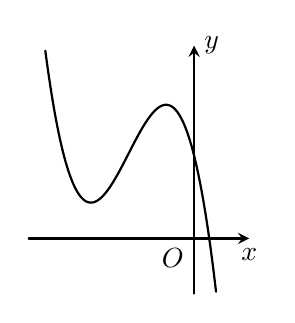
\begin{tikzpicture}[line join = round, line cap = round,>=stealth,thick,x = 1cm,y = 1cm,scale=.7] 
			%Vẽ hệ trục Oxy 
			\draw[->] (-3,0)--(0,0) node[below left]{$O$}--(1,0) node[below]{$x$}; 
			\draw[->] (0,-1)--(0,3.5) node[right]{$y$}; 
			%Vẽ đồ thị hàm số 
			\draw[samples=200,domain=-2.7:.4,smooth] plot (\x, {-1.4*(\x)^3-5*(\x)^2-4*\x+1.5}); 
		\end{tikzpicture}
} 
	\shortans{$1$}
	\loigiai{
		Ta có $y'=3a x^2+2bx+c$. \\
		Dựa vào đồ thị hàm số, ta nhận thấy
		\begin{itemize}
			\item  $a<0$.
			\item Giao điểm của đồ thị hàm số với trục tung là điểm $(0 ; d)$, suy ra $d>0$.
			\item Đồ thị hàm số có hai điểm cực trị nằm về bên trái trục $Oy$ nên ta cần có $y'=0$ có hai nghiệm âm phân biệt, nghĩa là
			$$
			\heva{&-\dfrac{2b}{3a}<0\\&b^2-3ac>0\\&\dfrac{c}{3a}>0} \Leftrightarrow \heva{&b^2-3ac>0\\&ab>0\\&ca>0} \Leftrightarrow\heva{&a<0\\&b<0\\& c<0\\&b^2-3ac>0}\text{ hoặc } \heva{&a>0\\&b>0\\&c>0\\&b^2-3ac>0.}
			$$
		\end{itemize}		
	Kết hợp lại ta có trong $4$ số $a$, $b$, $c$, $d$ chỉ có một số dương là $d$.
}
\end{ex}

\begin{ex}%[2D1V5-1]
	Cho hàm số $f(x)=\dfrac{ax+1}{bx+c}$, $(a$, $b$, $c \in \mathbb{R})$ có bảng biến thiên như sau
	\begin{center}
			
\begin{tikzpicture}
				\tkzTabInit[nocadre,lgt=1.2,espcl=5]
				{$x$/.7,$f’(x)$/.7,$f(x)$/2}
				{$-\infty$,$3$,$+\infty$}
				\tkzTabLine{ ,-,d,-,}
				\tkzTabVar{+/$-2$,-D+/$-\infty$/$+\infty$,-/$-2$}
			\end{tikzpicture}.
		\end{center}
	Trong các số $a$, $b$, $c$ có bao nhiêu số dương?
	\shortans{$1$}
	\loigiai{
	Tập xác định $\mathscr{D}=\mathbb{R} \setminus\{3\}$. Từ công thức của hàm số ta có
	\begin{itemize}
		\item $f'(x)=\dfrac{a c-b}{(b x+c)^2}$.
		\item Tiệm cận ngang của đồ thị hàm số $y=\dfrac{a}{b}$.
		\item Tiệm cận đứng của đồ thị hàm số $x=-\dfrac{c}{b}$.
	\end{itemize} 
	Mặt khác, dựa vào bảng biến thiên của hàm số ta có 
	\begin{itemize}
		\item $f'(x)<0$.
		\item Tiệm cận ngang của đồ thị hàm số $y=-2$.
		\item Tiệm cận đứng của đồ thị hàm số $x=3$.
	\end{itemize}
	Suy ra $\heva{&ac-b<0\\&\dfrac{a}{b}=-2\\ &-\dfrac{c}{b}=3} \Leftrightarrow\heva{&6b^2-b<0 \\ &a=-2b\\&c=-3b} \Leftrightarrow\heva{&0<b<\dfrac{1}{6}\\& -\dfrac{1}{3}<a<0 \\& -\dfrac{1}{2}<c<0.}$\\
	Vậy có $1$ số dương trong các số $a$, $b$, $c$.
	}
\end{ex}

\begin{ex}%[2D1V3-6]
	Anh A dự định sử dụng hết $4\, \mathrm{m}^2$ kính để làm một bể cá bằng kính có dạng hình hộp chữ nhật không nắp, chiều dài gấp đôi chiều rộng (các mối ghép có kích thước không đáng kể). Bể cá có thể tích lớn nhất bẳng bao nhiêu $\mathrm{m}^3$ (kết quả để ở dạng thập phân, làm tròn đến hàng phần trăm)?
	\shortans{$0{,}73$}
	\loigiai{
		\begin{center}
			\begin{tikzpicture}
				\def\a{3}
				\def\b{1}
				\def\g{30}
				\def\h{3}
				\path
				(0:0) coordinate (A)--++(\g:\b) coordinate (B)--++(0:\a) coordinate (C)--++(\g-180:\b) coordinate (D)
				\foreach \x in {A,B,C,D}{
					($(\x)+(90:\h)$) coordinate (\x')};
				\fill (A) circle (1pt) node [left] {$A$} (B) circle (1pt) node [above right] {$B$} (C) circle (1pt) node [right] {$C$} (D) circle (1pt) node [below right] {$D$} (A') circle (1pt) node [above left] {$A'$} (B') circle (1pt) node [above] {$B'$} (C') circle (1pt) node [above] {$C'$} (D') circle (1pt) node [below right] {$D'$};
				\draw ($(B)!.5!(C)$) node[above]{$2x$};
				\draw ($(C)!.6!(D)$) node[right]{$x$};
				\draw ($(D')!.5!(D)$) node[right]{$h$};
				\draw[dashed] (B')--(B)--(A)
				(B)--(C);
				\draw
				(A)--(D)--(D')--(A')--cycle
				(A')--(B')--(C')--(D')
				(D)--(C)--(C')
				;
			\end{tikzpicture}
		\end{center}
	Giả sử bể cá dạng hình hộp chữ nhật $ABCD.A'B'C'D'$ có kích thước như hình vẽ trên.\\
	Khi đó ta có diện tích xung quanh của bể cá là 
	$$S_{xq}=2\cdot S_{BCC'B'}+2\cdot S_{ABB'A'}=2 \cdot 2x\cdot h+2x\cdot h=4x\cdot h+2x\cdot h=6x\cdot h.$$
	Diện tích mặt đáy bể cá là $S_{ABCD}=2\cdot x\cdot  x=2x^2$.\\ 
	Theo đề bài ta có $2 x^2+6 x h=4 \Leftrightarrow h=\dfrac{4-2 x^2}{6 x}$.\\
	Do $x>0$, $h>0$ nên $4-2x^2>0 \Leftrightarrow 0<x<\sqrt{2}$.\\
	Mặt khác $V=2 x^2 h=\dfrac{4 x-2 x^3}{3}=f(x)$ với $x \in(0 ; \sqrt{2})$.\\
	Ta có $f'(x)=\dfrac{4}{3}-2 x^2$, $f'(x)=0 \Leftrightarrow \dfrac{4}{3}-2 x^2=0 \Leftrightarrow x=\dfrac{\sqrt{6}}{3}$ (vì $x>0$).\\
	Bảng biến thiên
	\begin{center}
		\begin{tikzpicture}
		\tkzTabInit[nocadre,lgt=2,espcl=3,deltacl=0.5]
		{$x$/1, $f(x)$/1, $f(x)$/2.5}
		{$-\infty$,$0$,$\tfrac{\sqrt{6}}{3}$,$\sqrt{2}$,$+\infty$}
		\tkzTabLine{,,,+,z,-,,,}
		\fill[pattern=north east lines]
		($(N13)+(-.5,0)$) rectangle (N21); 
		\fill[pattern=north east lines]
		(N43) rectangle ($(N43)+(3.5,3.5)$); 
		\draw (N23) node[above right] (A) {$0$} (N32) node [below] (B) {$\tfrac{8\sqrt{6}}{27}$} (N43) node[above left] (C){$0$};
		\draw[-stealth] (A)--(B);
		\draw[-stealth] (B)--(C);
	\end{tikzpicture}
	\end{center}
	Vậy bể cá có thể tích lớn nhất bằng $\dfrac{8 \sqrt{6}}{27} \approx 0{,}73 \,\mathrm{m}^3$.
	}
\end{ex}

\begin{ex}%[2D1C3-6] 
	Một người cần đi từ khách sạn $A$ bên bờ biển đến hòn đảo $C$. Biết rằng khoảng cách từ đảo $C$ đếnbờ biển là $10\, \mathrm{km}$, khoảng cách từ khách sạn $A$ đến điểm $B$ trền bờ gần đảo $C$ nhất là $40\, \mathrm{km}$. Người đó có thể đi đường thủy hoặc đi đường bộ rồi đi đường thủy (như hình vẽ sau). 
	\begin{center}
		\begin{tikzpicture}[line join = round, line cap = round,>=stealth,font=\footnotesize,scale=1]
			\draw (5,2.5)--(-1,0) node[below] {$A$} --(3,0) node[below] {$D$}-- (5,0)node[below] {$B$} --(5,2.5) node[below right] {$C$} circle (1cm)--(3,0);
			\fill (5,2.5) circle (1pt) node[above] {Hòn đảo};
			\fill (5,0) circle (1pt);
			\fill (-1,0) circle (1pt);
			\fill (3,0) circle (1pt);
		\end{tikzpicture}
	\end{center}
	Biết kinh phí đi đường thủy bằng thuyền là $5\, \mathrm{USD} / \mathrm{km}$, đi đường bộ bằng xe taxi là $3\, \mathrm{USD} / \mathrm{km}$. Hỏi người đó phải đi đường bộ một khoảng bao nhiêu km để kinh phí nhỏ nhất (kết quả để ở dạng thập phân)?
	\shortans{$32{,}5$}
\loigiai{
	Vi $B$ là điểm trên bờ gần hòn đảo $C$ nhất nên suy ra $BC \perp AB$.\\
	Theo đề bài, ta có $A B=40\,\mathrm{~km}$, $B C=10\,\mathrm{km}$.\\
	Gọi $D$ là điểm bất kì thuộc đoạn $AB$ ($D$ có thể trùng với $A$ hoặc $B$).\\
	Đặt $AD=x\,\mathrm{km}, x \in[0;40]$.\\
	Ta có $BD=40-x \Rightarrow D C=\sqrt{(40-x)^2+10^2}$.\\
	Để đi từ $A$ đến $C$, thì người đó có thể phải đi đường bộ trên đoạn $AD$ và đi đường thủy trên đoạn $DC$.\\
	Do đó tổng kinh phí đi từ $A$ đến $C$ là
		$$f(x)=3 x+5 \sqrt{(40-x)^2+10^2}=3 x+5 \sqrt{x^2-80 x+1700}\,\mathrm{USD}.$$
	Tập xác định của hàm số $y=f(x)$ là $\mathscr{D}=\mathbb{R}$.\\
	$f'(x)=3+5 \dfrac{2 x-80}{2 \sqrt{x^2-80 x+1700}}=\dfrac{3 \sqrt{x^2-80 x+1700}+5 x-200}{\sqrt{x^2-80 x+1700}}.$\\
	Ta có
	\begin{eqnarray*}
		f'(x)=0 &\Leftrightarrow& 3 \sqrt{x^2-80 x+1700}-200+5 x=0 \Leftrightarrow 3 \sqrt{x^2-80 x+1700}=200-5 x \\
		& \Leftrightarrow& \heva{&
			200-5 x \geq 0 \\&
			9\left(x^2-80 x+1700\right)=200-5 x}\Leftrightarrow x=\dfrac{65}{2} \in[0 ; 40].
	\end{eqnarray*}
	Bảng biến thiên
	\begin{center}
		
\begin{tikzpicture}
			\tkzTabInit[nocadre,lgt=1.2,espcl=4]
			{$x$/1,$f’(x)$/1,$f(x)$/2}
			{$0$,$\tfrac{65}{2}$,$40$}
			\tkzTabLine{ ,-,z,+, }
			\tkzTabVar{+/$f(0)$,-/$f\left(\tfrac{65}{2}\right) $ ,+/$f(40)$}
		\end{tikzpicture}
	\end{center}
	Dựa vào bảng biến thiên, hàm số $f(x)$ đạt giá trị nhỏ nhất trên $[0 ; 40]$ (tức là kinh phí nhỏ nhất) tại điểm $x=\dfrac{65}{2}$.\\ Vậy người đó phải đi đường bộ $\dfrac{65}{2} =32{,}5 \mathrm{~km}$ để kinh phí nhỏ nhất.
}
\end{ex}
\Closesolutionfile{ans}
\indapan{6}{ans/ans-2-B4-De1-KQ}